\documentclass[a4paper]{article}
%% Language and font encodings
\usepackage[english]{babel}
\usepackage[utf8x]{inputenc}
\usepackage[T1]{fontenc}
\usepackage{float}
%% Sets page size and margins
\usepackage[a4paper,top=3cm,bottom=2cm,left=3cm,right=3cm,marginparwidth=1.75cm]{geometry}
\usepackage[caption=false]{subfig}
%\setcounter{section}{-1}
%% Useful packages
\usepackage{fancyhdr}
\pagestyle{fancy}
\usepackage{amsmath}
\usepackage{amsthm}
\usepackage{enumitem}
\usepackage{eqnarray}
\usepackage{float}
\usepackage{esint}
\usepackage{wrapfig}
\usepackage{gensymb}
\usepackage{lipsum}
\usepackage{amssymb}
\usepackage{array}
\usepackage{tikz}
\usetikzlibrary{arrows,decorations.markings}
\usepackage[colorlinks=true, allcolors=blue]{hyperref}
\usepackage{graphicx}
\usepackage{amsmath}
\usepackage{amssymb}
\usepackage{graphicx}
\usepackage{mathtools}
\usepackage[colorlinks=true, allcolors=blue]{hyperref}
\DeclareMathOperator{\lcm}{lcm}
\DeclareMathOperator{\var}{Var}
\DeclareMathOperator{\sech}{sech}
\DeclareMathOperator{\cosech}{cosech}
\DeclareMathOperator{\cov}{Cov}
\DeclareMathOperator{\sgn}{sgn}
\DeclareMathOperator{\Span}{span}
\DeclareMathOperator{\nullity}{nullity}
\DeclareMathOperator{\rank}{rank}
\DeclareMathOperator{\Ker}{Ker}
\DeclareMathOperator{\R}{R}
\DeclareMathOperator{\Tr}{Tr}
\DeclareMathOperator{\sinc}{sinc}
\DeclareMathOperator{\diag}{diag}
\newtheorem{defi}{Definition}[section]
\newtheorem{remarks}{Remarks}[section]
\newtheorem{note}{Note}[section]
\newtheorem{law}{Law}[section]
\newtheorem{eg}{Example}[section]
\newtheorem{notation}{Notation}[section]
\newtheorem{thm}{Theorem}[section]
\newtheorem{prop}{Proposition}[section]
\newtheorem{lemma}{Lemma}[section]
\newtheorem{cor}{Corollary}[section]

\definecolor{darkblue}{RGB}{	0, 0, 139}
\newtheoremstyle{new}% <name>
{5pt}% <Space above>
{5pt}% <Space below>
{\color{black}}% Body font
{}% <Indent amount>
{\bfseries\color{darkblue}}% Theorem head font
{:}% <Punctuation after theorem head>
{.5em}% <Space after theorem headi>
{}% <Theorem head spec (can be left empty, meaning `normal')>
\theoremstyle{new}
\newtheorem{Note}{Note}[section]
\title{\textbf{TSP (Thermal and Statistical Physics) Part II Phy}}
\author{Tai Yingzhe, Tommy (ytt26)}
\date{}
\setlength{\parindent}{0cm}
\begin{document}
\maketitle
\tableofcontents
%\newpage
%The following are useful reference books:
%\begin{itemize}
    %\item Huang, Kerson. Statistical Mechanics. 2nd ed. Wiley, 1987. ISBN: 9780471815181.
    %\item Pathria, R. K. Statistical Mechanics. Pergamon Press, 1972. ISBN: 9780080189949.
    %\item Pippard, A. B. The Elements of Classical Thermodynamics for Advanced Students of Physics. University Press, 1966.
    %\item Ma, Shang-keng. Statistical Mechanics. Translated by M. K. Fung. World Scientific Publishing Company, 1985. ISBN: 9789971966065.
    %\item Landau, L. D., and E. M. Lifshitz. Statistical Physics, Part 1. 3rd ed. Pergamon Press, 1980. ISBN: 9780080230382.
    %\item Reif, Frederick, ed. Fundamentals of Statistical and Thermal Physics. McGraw-Hill, 1965.
    %\item Kardar, Mehran. Statistical Physics of Particles. Cambridge University Press, 2007. ISBN 9780521873420.
    %\item Kardar, Mehran. Statistical Physics of Fields. Cambridge University Press, 2007. ISBN: 9780521873413.
    %\item  Ma, Shang-keng. Modern Theory of Critical Phenomena. Addison-Wesley, 1976. ISBN: 9780805366709.
    %\item H. Eugene. Introduction to Phase Transitions and Critical Phenomena. Oxford University Press, 1993. ISBN: 9780195014587.
    %\item Amit, Daniel J. Field Theory, the Renormalization Group, and Critical Phenomena. Revised 2nd ed. World Scientific Publishing Company, 1984. ISBN: 9789971966102.
    %\item Negele, John W., and Henri Orland. Quantum Many-particle Systems.Perseus Books, 1988. ISBN: 9780201125931.
    %\item Parisi, Giorgio. Statistical Field Theory. Addison-Wesley, 1988. ISBN: 9780201059854.
%\end{itemize}

\newpage
\section{Recap of Thermodynamics}
\subsubsection*{Definitions}
\begin{defi}[Thermodynamic System]
A thermodynamic system contains an arbitrary amount of matter and may allow exchange with the surroundings.
\end{defi}
\begin{defi}[Isolated Systems]
Isolated systems do not interact in any way with the surroundings. Here, energy and particle number are conserved quantities. 
\end{defi}
\begin{defi}[Closed Systems]
Closed systems can only exchange energy with their surroundings. Energy is not conserved; if the system is in equilibrium with its surroundings, mean value of energy is related to the temperature of the system or the surroundings.
\end{defi}
\begin{defi}[Open Systems]
Open systems can exchange energy and matter with their surroundings; energy and particle number are not conserved; if the system is in equilibrium with its surroundings, mean values of energy and the particle number are related to the temperature and chemical potential of the system or of the surroundings.
\end{defi}
\begin{defi}[Thermodynamic Equilibrium State]
Thermodynamic equilibrium state is defined as the one macroscopic state of a system which is automatically attained after a sufficiently long period of time such that the macroscopic properties of the system no longer change with time.
\end{defi}
\begin{defi}[Thermal Equilibrium]
A system is said to be in thermal equilibrium if there is no temperature difference between system and surroundings.
\end{defi}
\begin{defi}[Mechanical Equilibrium]
A system is said to be in mechanical equilibrium if there is no unbalanced forces acting on any part of the system or the system as a whole.
\end{defi}
\begin{defi}[Diffusive Equilibrium]
A system is said to be in diffusive equilibrium if there is no chemical reaction within the system and there is no movement of particles from one part of the system to the other.
\end{defi}
\begin{defi}[Thermodynamic State Functions]
Thermodynamic state functions are macroscopic quantities which describe the system. The state functions are only well-defined and measurable when the system is in equilibrium.
\end{defi}
\begin{defi}[Equation of State]
Equation of state gives a mathematical relationship between thermodynamic state functions. Equation of state is specified empirically in thermodynamics but is derived theoretically in statistical mechanics.
\end{defi}
\begin{defi}[Extensive Quantities]
Extensive quantities are proportional to the amount of matter in a system.
\end{defi}
\begin{defi}[Intensive Quantities]
Intensive quantities are independent of the amount of matter in a system.
\end{defi}
\begin{defi}[Conjugate Pair Variables]
$(T,P,\mu)$ are intensive variables which form a conjugate pair with $(S,V,n)$, which are extensive variables, respectively. 
$$\mu=\frac{\partial U}{\partial n},\quad T=\frac{\partial U}{\partial S},\quad P=-\frac{\partial U}{\partial V}$$
If one applies a constraint to the given system, then the corresponding conjugate variable will change as a response.
\end{defi}
\newpage
\subsubsection*{Zeroth Law and First Law}
\begin{law}[Zeroth Law of Thermodynamics]
If two systems are separately in thermal equilibrium with a third, then they must also be in thermal equilibrium with each other.
\end{law}
\begin{defi}[Temperature]
Temperature, a state function, describes the tendency of a system to exchange energy with other system. An empirical state function whose existence is implied from the zeroth law.
\end{defi}
\begin{cor}
All systems in thermal contact have the same temperature when in thermal equilibrium and no energy is exchanged between them. Otherwise, energy is transferred from the hotter system to the colder system.
\end{cor}
\begin{defi}[Energy]
Energy of the system is the sum of two contributions:
\begin{itemize}
    \item For the macroscopic motion of the system, i.e. the kinetic energy of the motion of the centre of mass of the system, and the potential energy of the system due to the presence of external fields. 
    \item Internal energy of the system: sum of the energy of all the internal degrees of freedom, which include the sum of the kinetic energy of the particles in the system in the reference frame in which the centre of mass is at rest, as well as, the potential energy arising from the interactions of the particles in the system.
\end{itemize}
The first contribution is ignored in thermal physics. The internal energy is an extensive state function and depends only on the equilibrium state of the system, described by a set of state functions.
\end{defi}
\begin{defi}[Ideal Gas]
Ideal gas is a collection of non-interacting point-like particles with equation of state $PV=Nk_BT=nRT$, where $k_B=\frac{R}{N_A}$, where $N_A$ is the Avogadro number. The internal energy of an ideal gas is only dependent on its temperature.
\end{defi}
\begin{defi}[Heat]
Heat is the energy flow between a system and its surroundings due to a temperature difference across the wall (which partitions the system from its surroundings), and a finite thermal conductivity of the wall.
\end{defi}
\begin{defi}[Work]
Work is any other kind of energy across the wall of the system.
\end{defi}
\begin{cor}
Both heat and work are not state functions and depend on the nature of the process transferring energy to the system.
\end{cor}
\begin{law}[First Law of Thermodynamics]
Energy, i.e. internal energy $U$, is conserved and is transferred between systems as either heat $Q$ or work $W$
$$dU=\delta Q+\delta W$$
where $dU$ is an exact differential but $\delta Q$ and $\delta W$ are inexact differentials. They are conventionally positive if energy flows into the system.
\end{law}
\begin{defi}[Reversible Process]
A process is reversible if it is possible to restore the system and its surroundings to their original conditions.
\end{defi}
\begin{defi}[Quasi-Static Process]
A process is quasi-static if it is sufficiently slow such that any intermediate state can be considered as an equilibrium state. They can be specified by a mathematical curve $\mathcal{C}$ as a function of state functions.
\end{defi}
\begin{eg}
Examples of quasi-static processes:
\begin{itemize}
    \item Isobaric: constant pressure
    \item Isochoric: constant volume
    \item Isothermal: constant temperature
    \item Adiabatic: zero heat transfer, especially when system is thermally isolated from surroundings.
\end{itemize}
\end{eg}
\begin{defi}[Quasi-Static Work]
Quasi-static work can be regarded as a product of generalized displacement and their conjugate generalized forces. Former is usually extensive while latter are intensive.
\end{defi}
\begin{eg}
Labelling generalized force and displacement as an ordered tuple, 
\begin{itemize}
    \item Film: Surface Tension and Area
    \item Magnet: Magnetic Field and Magnetization
    \item Dielectric: Electric Field and Polarization
    \item Chemical Reaction: Chemical Potential and Particle Number
\end{itemize}
\end{eg}
\begin{defi}[Response Functions]
Response functions are used to characterize the macroscopic behaviour of a system and are experimentally measured from the changes of thermodynamic state functions with external probes.
\end{defi}
\begin{defi}[Heat Capacity]
Heat capacity is an extensive quantity which describes the change in the temperature of the system resulting from a transfer of heat,i.e. $C=\frac{\partial Q}{\partial T}$ The nature of heat process is to be specified. To make this quantity intensive, we divide it by number of moles or by mass.
\end{defi}
\begin{defi}[Thermal Responses]
Thermal responses probe the change in the thermodynamic state function with temperature.
\end{defi}
\begin{defi}[Expansivity]
Expansivity measures the fractional change in volume with a change in temperature.
\end{defi}
\begin{defi}[Force Constants]
Force constants probe the change in the thermodynamic state function with force.
\end{defi}
\begin{defi}[Compressibility]
Compressibility is the fractional change in volume when a force is applied, multiplied by a negative sign.
\end{defi}
\begin{eg}
For ideal gas, $PV=nRT$, we have expansivity $\beta_P=\frac{1}{V}(\frac{\partial V}{\partial T})_P=\frac{1}{T}$ and compressibility $\kappa_T=-\frac{1}{V}(\frac{\partial V}{\partial P})_T=\frac{1}{P}$.
\end{eg}
\begin{prop}
For an ideal gas, the heat capacities satisfy the relation
$$C_P-C_V=nR$$
\end{prop}
\begin{eg}[Paramagnetic salt in an applied magnetic field]
The work required to change the magnetic moment of a substance from $\mathbf{m}$ to $\mathbf{m}+d\mathbf{m}$ in an applied external field $\mathbf{H}$ conventionally regards only the work needed to change the state of the substance, returning any external sources of field back to zero. A paramagnetic substance with magnetic moment $\mathbf{m}(\mathbf{H})$ at some large distance from a permanent magnet will experience an attractive force $(\mathbf{m}\boldsymbol{\nabla})\mathbf{H}$. Letting the substance approach the magnet until it experiences a field $\mathbf{H_1}$, we can extract work, so that the work done on the substance is $W'=-\mu_0\int_0^{H_1}\mathbf{m}(\mathbf{H})d\mathbf{H}$. However, the magnet is still near the substance, so in order to calculate the work required to change the state of the substance alone, we need to pull the magnet away to the previous separation, while keeping the magnetic moment $\mathbf{m_1}$ constant, i.e. $W_1=\mu_0\int_0^{H_1}\mathbf{m_1}dH=\mu_0m_1H_1$. This gives a net work $W=\mu_0\int\mathbf{H} d\mathbf{m}$.\\[5pt]
The difference between the two expressions is the change in the potential energy of the dipole moment in an applied field, $-\mu_0d(mH)$, which is conventionally not counted as part of the internal energy. 
\end{eg}
\newpage
\subsubsection*{Real Gases}
\begin{defi}[van der Waals Gas]
The equation of state for a van der Waals gas is
$$\bigg(p-\frac{a}{V_m^2}\bigg)(V_m-b)=RT$$
where $V_m$ is the molar volume, $a$ parametrizes the strength of the inter-molecular interactions while $b$ is the volume excluded owing to the finite size of the molecules.
\end{defi}
\begin{Note}[Derive equation of state]
Assuming $n$ moles of gas in volume $V$, the number of nearest neighbours is proportional to $n/V$, and so the attractive intermolecular interactions lower the total potential energy by an amount proportional to the number of atoms multiplied by the number of nearest neighbours. Changing $V$, the energy changes by an amount $an^2dV/V^2$. This energy change can be thought of as being due to an effective pressure $p_{eff}$, i.e. $-p_{eff}dV$, hence $p_{eff}=-\frac{a}{V_m^2}$. The pressure that you measure is the sum of the ideal pressure and effective pressure, so $p_{ideal}=p+\frac{a}{V_m^2}$.\\[5pt]
We can estimate $b$ by simple hard sphere model. Each molecule excludes a spherical volume $\frac{4}{3}\pi(2r)^3$ and for one mole, $b=\frac{1}{2}N_A\frac{4}{3}\pi(2r)^3=\frac{16}{3}N_A\pi r^3$. The factor 0.5 arises because the key situation is when a collision occurs - so one considers how much space is `off limits' for a pair of atoms.
\end{Note}
\begin{Note}[van der Waals' Isotherms]
Starting at the low density side (i.e., high volume $v$ per particle), we find behaviour approaching that of an ideal gas. As the density increases, the inter-molecular attraction term $N^2a/V^2$ causes the isotherm to fall below the ideal gas pressure, until we start to approach the density of closest packing, at which point the hard core repulsion term $N b$ causes the pressure to skyrocket. On some isotherms there is a very odd region where $\partial p/\partial V$ is positive, a situation which is mechanically unstable.\\[5pt]
The isotherms can be obtained via the cubic equation
$$pV^3-(pb+RT)V^2+aV-ab=0$$
At high $T$, $pV_m=RT$ is a good approximation. C is a point of inflection, denoting the critical temperature, and the point is on the critical isotherm. For $T<T_c$, the isotherms exhibit a S-shape curve with a minimum and a maximum. There is a region in which the isothermal compressibility $\kappa_T=-\frac{1}{V}(\frac{\partial V}{\partial p})_T$ is negative, i.e. compressing the gas increases the volume.\\[5pt]
The dashed curve with maximum at critical point, represents phase equilibrium between vapor and liquid. The region bounded by the curve is a 2-phase, for small $V$ on the left outside the region is a liquid and for large $V$ on the right, it is a vapor.
\end{Note}
\begin{prop}[Critical Point]
At the critical point, $\frac{p_cV_c}{RT_c}=\frac{3}{8}$.
\end{prop}
\begin{proof}
Since $p=\frac{RT}{V-b}-\frac{a}{V^2}$ and at the critical point, we require both
$$\bigg(\frac{\partial p}{\partial V}\bigg)_T=\frac{-RT}{(V-b)^2}+\frac{2a}{V^3}=0,\quad \bigg(\frac{\partial^2 p}{\partial V^2}\bigg)_T=\frac{2RT}{(V-b)^3}-\frac{6a}{V^4}=0$$
to be true. This yields $V_c=3b$ and hence $T_c=\frac{8a}{27Rb}$. The corresponding critical pressure is $p_c=\frac{a}{27b^2}$. The compressibility factor is $\frac{p_cV_c}{RT_c}=\frac{3}{8}$, independent of both $a$ and $b$. Moreover, at this point, the isothermal compressibility diverges.
\end{proof}
\newpage
\subsection*{Entropy}
\begin{defi}[Heat Reservoirs]
Heat reservoirs are systems with a fixed tendency to exchange energy, i.e. fixed temperatures.
\end{defi}
\begin{defi}[Ideal Heat Engine]
A heat engine is a cyclic process in a system that absorbs heat $Q_{in}$, rejects heat $Q_{out}$, and a positive amount of work $|W|$ is done by the engine. The heat transferred to the system in one cycle is $Q=-W$ since $\Delta U=0$. The efficiency of the heat engine is 
$$\eta=\frac{|W|}{Q_{in}}=1-\frac{|Q_{out}|}{|Q_{in}|},\quad0\leq\eta\leq 1$$
\end{defi}
\begin{defi}[Refrigerator]
A refrigerator is a heat engine that is run backwards so that you put work in and cause a heat flow from a cold reservoir to a hot reservoir. Another name is a heat pump.
\end{defi}
\begin{law}[Clausius Statement of Second Law of Thermodynamics]
There is no process whose only effect is to accept heat from a colder reservoir and transfer it to a hotter reservoir.
\end{law}
\begin{law}[Kelvin Statement of Second Law of Thermodynamics]
There is no process whose only effect is to accept heat from a single heat reservoir and convert it entirely into work.
\end{law}
\begin{figure}[H]
    \centering
    \includegraphics[scale=0.8]{secondlaw1.PNG}
    \caption{Clausius and Kelvin Engine. \cite{blundell2010concepts}}
\end{figure}
\begin{thm}
The Kelvin and Clausius statements of the Second Law of Thermodynamics are equivalent.
\end{thm}
\begin{proof}
We first show that if Clausius statement is not true, then it implies that Kelvin statement is not true. Suppose there exists a Clausius-violating device (accepts $|Q_2|$ heat from cold reservoir and dump the exact same amount to the hotter reservoir), that acts together with a heat engine (accepts heat $|Q_1|-|Q_2|$ from a single heat reservoir at temperature $T_1$ and converting it entirely into work $|W|=|Q_1|-|Q_2|$). This combined system violates Kelvin's statement since the heat accepted from the hotter reservoir is completely converted to work.\\[5pt]
Conversely, suppose there exists a Kelvin-violating device (converting heat $|Q_1'|$ entirely into work $|W|$), that acts together with a refrigerator, accepts heat $|Q_2|$ from a colder reservoir at temperature $T_2$ and transfer heat $|Q_1|$ to a hotter reservoir at temperature $T_1$. The combined system violates Clausius' statement since it takes heat $|Q_2|$ from a colder reservoir and dumps heat $|Q_2|=|Q_1|-|Q_1'|>0$ onto a hotter reservoir.
\end{proof}
\begin{figure}[H]
    \centering
    \includegraphics[scale=0.8]{secondlaw2.PNG}
    \caption{(Top) First part of proof. (Bottom) Second part of proof. \cite{blundell2010concepts}}
\end{figure}
\begin{defi}[Carnot Engine]
Carnot engine is an idealized system that is cyclic and reversible with all of its heat exchanges taking place at a hotter reservoir at temperature $T_1$ and a colder reservoir at temperature $T_2$.
\end{defi}
\begin{defi}[Ideal Refrigerator]
An ideal refrigerator is a Carnot cycle run in reverse.
\end{defi}
\begin{defi}[Carnot Cycle]
Carnot Cycle consists of 4 processes:
\begin{enumerate}
    \item A to B: isothermal expansion at $T_1$
    \item B to C: adiabatic expansion to $T_2$
    \item C to D: isothermal compression at $T_2$
    \item D to A: adiabatic compression to $T_1$.
\end{enumerate}
\begin{center}
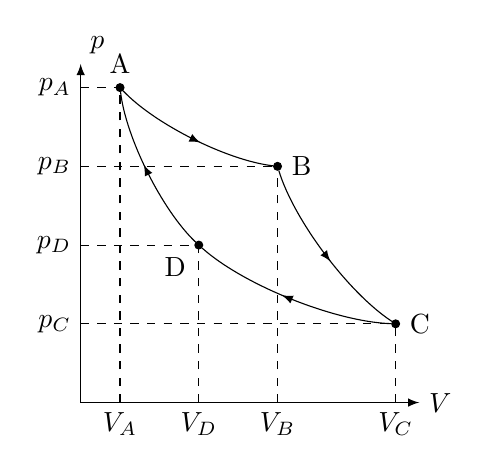
\begin{tikzpicture}[
  > = latex,
  dot/.style = {draw,fill,circle,inner sep=1pt},
  arrow inside/.style = {postaction=decorate,decoration={markings,mark=at position .55 with \arrow{>}}}
  ]
  \draw[<->] (0,4.3) node[above right] {$p$} |- (4.3,0) node[right] {$V$};
  \node[dot,label={above:A}] (@1) at (0.5,4) {};
  \node[dot,label={right:B}] (@2) at (2.5,3) {};
  \node[dot,label={right:C}] (@3) at (4,1) {};
  \node[dot,label={below left:D}] (@4) at (1.5,2) {};
  \draw[arrow inside] (@1) to[looseness=.7,bend right=20] (@2);
  \draw[arrow inside] (@2) to[looseness=.7,bend right=20] (@3);
  \draw[arrow inside] (@3) to[looseness=.7,bend left=20] (@4);
  \draw[arrow inside] (@4) to[looseness=.7,bend left=20] (@1);
  \draw[dashed,thin] (0,4) node[left] {$p_A$} -- (0.5,4);
  \draw[dashed,thin] (0.5,0) node[below] {$V_A$} -- (0.5,4);
  \draw[dashed,thin] (0,3) node[left] {$p_B$} -- (2.5,3);
  \draw[dashed,thin] (2.5,0) node[below] {$V_B$} -- (2.5,3);
  \draw[dashed,thin] (0,1) node[left] {$p_C$} -- (4,1);
  \draw[dashed,thin] (4,0) node[below] {$V_C$} -- (4,1);
  \draw[dashed,thin] (0,2) node[left] {$p_D$} -- (1.5,2);
  \draw[dashed,thin] (1.5,0) node[below] {$V_D$} -- (1.5,2);
\end{tikzpicture}
\end{center}
\end{defi}
\begin{thm}
The energy efficiency of Carnot engine with ideal gas as a working substance is $$\eta=1-\frac{T_2}{T_1}$$
\end{thm}
\begin{proof}
Since A to B is an isothermal expansion, C to D is an isothermal compression, then we have
$$|Q_{in}|=Q_{A\rightarrow B}=nRT_1\ln(V_B/V_A)$$
$$|Q_{out}|=-Q_{C\rightarrow D}=-nRT_2\ln(V_D/V_C)$$
Then the efficiency is $\eta=1-\frac{|Q_{out}|}{|Q_{in}|}=1-\frac{T_2}{T_1}\frac{\ln(V_D/V_C)}{\ln(V_A/V_B)}$. Since $TV^{\gamma-1}$ is a constant for adiabatic processes, then $V_C/V_B=V_D/V_A$ and so $\eta=1-\frac{T_2}{T_1}$.
\end{proof}
\begin{cor}
For Carnot engine, $\frac{|Q_{out}|}{|Q_{in}|}=\frac{T_2}{T_1}$
\end{cor}
\begin{thm}[Carnot's Theorem]
No engine operating between two reservoirs can be more efficient than a Carnot engine operating between the same two reservoirs.
\end{thm}
\begin{proof}
Suppose we have a hypothetical super-efficient engine SE and Carnot refrigerator CR, such that $\eta_{SE}>\eta_{CR}\implies|Q_1|>|Q_1'|$ and hence $W=|Q_1'|-|Q_2'|=|Q_1|-|Q_2|$ and hence $|Q_1|-|Q_1'|>0$ is the amount of heat dumped into the hotter reservoir while $|Q_2|-|Q_2'|>0$ is the amount of heat extracted from the colder reservoir. This violates Clausius statement.
\end{proof}
\begin{cor}
All Carnot engines operating between the same two reservoirs have the same efficiency.
\end{cor}
\begin{proof}
Prove this by setting up $\eta_1\leq\eta_2$ and $\eta_2\leq\eta_1$ and pay attention to Carnot's Theorem and Clausius' statement.
\end{proof}
\begin{figure}[H]
    \centering
    \includegraphics[scale=0.7]{secondlaw3.PNG}
    \caption{(left) Demonstrates Carnot's Theorem. (centre and right) for Corollary. \cite{blundell2010concepts}}
\end{figure}
\begin{defi}[Empirical Temperature]
Carnot's theorem means that the ratio of the heat transfers into and out of the hot and cold reservoirs is a function of the temperature of the reservoirs only. It is thus imperative to define an empirical temperature to be the ratio of heat transfers, i.e. $\frac{Q_2}{Q_1}=f(T_1,T_2)$ where $Q_1$ is heat supplied to the cold reservoir $T_1$ and $Q_2$ is heat extracted from the hot reservoir $T_2$.
\end{defi}
\begin{thm}[Clausius Inequality]
For a general cycle, reversible or not, the relation $$\oint\frac{dQ}{T}\leq 0$$ is true.
\end{thm}
\begin{proof}
Suppose heat $\delta Q_i$ at each point of a general cycle is supplied via a Carnot engine, which is connected between a reservoir at temperature $T$ and the reservoir at temperature $T_i$. The reservoir at $T$ is common for all the Carnot engines connected at all points of the cycle.\\[5pt]
Each Carnot engine produces work $\delta W_i$ and for a Carnot engine, we know that $\frac{\delta Q_i}{T_i}=\frac{\delta Q_i+\delta W_i}{T}$. The total work extracted from the cycle is $\Delta W=\sum_{cycle}\delta Q_i$. And so the total work produced per cycle is $\Delta W+\sum_{cycle}\delta W_i\leq 0$.
$$\sum_{cycle}\delta Q_i+\sum_{cycle}\delta Q_i\bigg(\frac{T}{T_i}-1\bigg)\leq0\implies \sum_{cycle}\frac{\delta Q_i}{T_i}\leq 0$$
since $T>0$. Changing the sum to a closed loop path integral, we obtain the Clausius' inequality.
\end{proof}
\begin{cor}
For reversible cycle, $\oint\frac{dQ}{T}=0$.
\end{cor}
\begin{defi}[Entropy]
Entropy, denoted as $S$, is $$dS=\frac{\delta q_{rev}}{T}$$ where $\delta q_{rev}$ is an infinitesimal amount of heat absorbed in a reversible process. 
\end{defi}
\begin{thm}[Second Law of Thermodynamics]
An equivalent statement of the Second Law of Thermodynamics states that for a thermally isolated system,
$$dS\geq0$$
In particular, $dS=0$ for a reversible process and $dS>0$ for an irreversible process.
\end{thm}
\begin{proof}
Consider a loop which contains an irreversible section A to B and a reversible section B to A. By Clausius' inequality, we have
$$dS=\frac{\delta q_{rev}}{T}\geq\frac{\delta q}{T}$$
For a thermally isolated system, we have $\delta q=0$. So, $dS\geq0$ in general.
\end{proof}
\begin{defi}[Entropy Change of Surroundings and System]
Since the surroundings (i.e. a heat reservoir) is much larger than the system, the temperature of the surroundings does not change, despite the heat transfer. This heat transfer, as seen from the point of view of the surroundings, is reversible, hence $\Delta q_{surr}=\Delta q_{surr,rev}$. Moreover, since energy is conserved, $\Delta q_{surr}=-\Delta q_{sys}$
$$\Delta S_{surr}:=\frac{\Delta q_{surr,rev}}{T_{surr}}=\frac{\Delta q_{surr}}{T_{surr}}=\frac{-\Delta q_{sys}}{T_{surr}}$$
As for the system, from the definition of entropy:
$$\Delta S_{sys}=\frac{q_{rev,sys}}{T}$$
This is true for both reversible and irreversible process.
\end{defi}
\begin{defi}[Equilibrium]
A system is said to be in equilibrium if $dS_{univ}=0$.
\end{defi}
\begin{defi}[Spontaneity]
A spontaneous process occurs when the resultant change in entropy of the Universe is positive, i.e. $dS_{univ}>0$. Note that
$$\Delta S_{univ}=\Delta S_{surr}+\Delta S_{sys}$$
\end{defi}
\begin{Note}[Reversible Expansion Versus Irreversible Expansion]
In general, expansion occurs when $p_{internal}>p_{external}$. Whenever there is a constant external pressure imposed on the system of gas, the expansion is said to be irreversible. It is also known as Joule expansion. It is spontaneous and system will tend towards mechanical equilibrium where $p_{internal}=p_{external}$.\\[5pt]
In contrast, for a reversible expansion, the external pressure is infinitesimally greater than the internal pressure. Any infinitesimal change in the external pressure will thus change the direction of the process. Such a process is infinitely slow since it is at equilibrium.
\end{Note}
\begin{Note}[Internal Energy as Extensive Function]
Since internal energy is extensive, i.e. depends linearly on the size of the system, then $U(\lambda S, \lambda X)$, where $X$ are all other possible extensive variables (could be generalized). Then, $U(\lambda S,\lambda X)=\lambda U(S,X)$. Thus, $U(S,X)$ is a first-order homogeneous function of $S$ and $X$.
\end{Note}
\newpage
\subsubsection*{Potentials}
\begin{defi}[Thermodynamic Potentials]
Since internal energy is the sum of $\delta q$ and $\delta W$, it can be written as
$$dU=TdS-pdV$$
where $S$ and $V$ are natural variables of $U$, such that we denote $U$ as $U(S,V)$. We correspondingly define three more thermodynamic potentials: enthalpy $H$, Gibbs function $G$ and Helmholtz function $F$
$$H=U+PV\implies dH=dU+d(pV)=TdS-pdV+pdV+Vdp=TdS+Vdp$$
$$G=H-TS\implies dG=dH-d(TS)=TdS+Vdp-TdS-SdT=-SdT+Vdp$$
$$F=U-TS\implies dF=dU-d(TS)=TdS-pdV-TdS-SdT=-SdT-pdV$$
The natural variables are thus $H(S,p)$, $F(T,V)$, $G(p,T)$. Note that here we take $N$ to be fixed. Otherwise, we have $F(T,V,N)$, $G(p,T,N)$, $H(S,p,N)$ and $U(S,V,N)$. Physically, they mean:
\begin{itemize}
    \item Internal Energy: energy needed to create a system;
    \item Enthalpy: energy needed to create a system plus the work needed to make room for it;
    \item Gibbs Free Energy: energy needed to create a system and make room for it minus the energy you can get from the environment;
    \item Helmholtz Free Energy: energy needed to create a system minus the energy you can get from the environment.
\end{itemize}
\end{defi}
\begin{defi}[Legendre Transformation]
A Legendre transform converts from a function of one set of variables to another function of a conjugate set of variables. 
\end{defi}
\begin{thm}
The Legendre transform of $f=f(x_1,...,x_n)$ is $g=f-\sum_{i=r+1}^nu_ix_i$, where $u_i=(\frac{\partial f}{\partial x_i})_{x_j}$, such that $g=g(x_1,...,x_r,u_{r+1},...,u_n)$ where $u_{r+1},...,u_n$ are conjugate variables to $x_{r+1},...,x_n$.
\end{thm}
\begin{proof}
We evaluate $dg$
$$dg=df-\sum_{i=r+1}^n(u_xdx_i+x_idu_i)=\sum_{i=1}^ru_idx_i+\sum_{i=r+1}^n(-x_i)du_i$$
$g$ is indeed a function of $x_i$ for $i\in[1,r]$ and $u_i$ for $i\in[r+1,n]$.
\end{proof}
\begin{cor}
The thermodynamic potentials can be inter-converted from Legendre Transformation.
\end{cor}
\begin{proof}
Since $T=(\frac{\partial U}{\partial S})_V$ and $p=-(\frac{\partial U}{\partial V})_S$, then $(T,S)$ and $(p,-V)$ are conjugate variables pair. To construct $F$ from $U$, we subtract the quantity $S$ times the variable conjugate to $S$, which is $T$, i.e. $F=U-TS$. Similarly, to construct $H$ from $U$, we subtract the quantity $V$ with its conjugate, which is $-p$, i.e. $H=U-(-pV)$. Lastly, to construct $G$ from $U$, we first convert it to $F$ and then deduct $-pV$. 
\end{proof}
\begin{thm}[Maxwell's Relations]
$$\bigg(\frac{\partial T}{\partial V}\bigg)_S=-\bigg(\frac{\partial p}{\partial S}\bigg)_V,\quad\bigg(\frac{\partial T}{\partial p}\bigg)_S=-\bigg(\frac{\partial V}{\partial S}\bigg)_p,\quad\bigg(\frac{\partial p}{\partial T}\bigg)_V=-\bigg(\frac{\partial S}{\partial V}\bigg)_T,\quad\bigg(\frac{\partial V}{\partial T}\bigg)_p=-\bigg(\frac{\partial S}{\partial p}\bigg)_T$$
\end{thm}
\begin{proof}
For all four, we use Clairaut's theorem (symmetry of second partial derivatives). The first, second, third and fourth were obtained from $U$, $H$, $F$ and $G$ respectively.\\[5pt]
Alternatively, one may use Jacobian. Consider a cyclic process that can be described in both the T-S and p-V plane. The internal energy $U$ is a state function and therefore doesn't change in a cycle and since $\oint dU=0$, we have $\oint pdV=\oint TdS$ and so $\frac{\partial(T,S)}{\partial(p,V)}=1\implies\frac{\partial(T,S)}{\partial(x,y)}=\frac{\partial(p,V)}{\partial(x,y)}$ where $(x,y)$ can be taken as $(T,p)$, $(T,V)$, $(p,S)$ and $(S,V)$ respectively.
\end{proof}
In general, there are more than 4 Maxwell's relations. Given a particular thermodynamic potential, expressed in terms of its $(1+r+s)$ natural variables, there are $(1+r+s)(r+s)/2$ distinct pairs of mixed second derivatives yielding $(1 + r + s)(r + s)/2$ Maxwell’s relations.
\begin{cor}
$dU$ gives the heat transfer $\delta q$ to a system at constant $V$ while $dH$ gives the heat transfer $\delta q$ to a system at constant $p$, i.e. energetics of a chemical reaction.
\end{cor}
Proof is trivial. Note that only $pV$ type of work can be involved.
\begin{thm}[Gibbs-Helmholtz Equations]
$$U=-T^2\bigg(\frac{\partial}{\partial T}\frac{F}{T}\bigg)_V,\text{    }H=-T^2\bigg(\frac{\partial}{\partial T}\frac{G}{T}\bigg)_P$$
\end{thm}
\begin{proof}
Using the expressions $S=-(\frac{\partial F}{\partial T})_V$ and $S=-(\frac{\partial G}{\partial T})_p$, we get
$$U=F+TS=F-T\bigg(\frac{\partial F}{\partial T}\bigg)_V=-T^2\bigg(\frac{\partial}{\partial T}\frac{F}{T}\bigg)_V$$
$$H=G+TS=G-T\bigg(\frac{\partial G}{\partial T}\bigg)_p=-T^2\bigg(\frac{\partial}{\partial T}\frac{G}{T}\bigg)_p$$
\end{proof}
\begin{thm}
The following statements are true:
\begin{itemize}
    \item At constant entropy, i.e. reversible adiabatic change, the work done by a system is equal to $dU$.
    \item At constant temperature, the maximum amount of energy which can be converted to work is given by $-dF$.
    \item At constant temperature and pressure, the maximum amount of energy which can be converted to non-$pV$ work is given by $dG$.
\end{itemize}
\end{thm}
\begin{proof}
First one is trivial, since $dU=-pdV$. For second one, since
$$dF=\delta q_{sys}+\delta W-TdS-SdT$$
and the $\delta q_{sys}=-\delta q_{res}$, then at constant temperature,
$$dF=\delta W-T(dS_{res}+dS)=\delta W-TdS_{total}\implies -\delta W=-dF-TdS_{total}\leq -dF$$
The maximum amount of energy which can be converted to work, occurs when $dS_{total}=0$. For third one, since at constant temperature and pressure,
$$dG=\delta q_{sys}+\delta W+pdV−TdS$$
when the change is reversible, $\delta q_{sys}=TdS$. Furthermore, $\delta W=-pdV+\delta W_{nonPV}$ and so $\delta G=\delta W_{nonpV}$ and this maximum conversion occurs in a reversible process.
\end{proof}
\begin{cor}
The following statements are true:
\begin{itemize}
    \item At constant temperature and volume, as well as, no non-$pV$ work present, $F$ must be minimized to find the equilibrium state.
    \item At constant pressure and volume, as well as, no non-$pV$ work present, $G$ must be minimized to find the equilibrium state.
\end{itemize}
\end{cor}
\begin{proof}
We have from earlier, $dF=-TdS_{tot}$. Since from Second Law of thermodynamics, we have $dS_{tot}>0$, we have $dF<0$. Similarly, $dG=-TdS_{tot}$ and hence $dG<0$.
\end{proof}
\begin{defi}[Availability]
The availability of a given system is defined as the maximum useful work that can be obtained in a process in which the system comes to equilibrium with the surroundings. 
$$A=U+p_0V-T_0S$$
where $p_0$ and $T_0$ are constants.
\end{defi}
\begin{cor}
For a mechanically isolated system, $dA\leq 0$ regardless of any other further constraints. 
\end{cor}
\begin{proof}
For a thermally isolated system of fixed volume, $dU=0$ and $dV=0$ and so $dA=-T_0dS$. Since $dS\geq0$ from second law, we obtain $dA\leq 0$ as desired.\\[5pt]
If instead the system was at fixed volume and fixed temperature, $dT=0$ and $dV=0$, then $dA=dU-T_0dS$ which is equal to $dF=dU-T_0dS-SdT=dU-T_0dS$. Hence, $dA=dF\leq0$.\\[5pt]
Lastly, if the system was at constant pressure and temperature, $dp=dT=0$, we have $dA=dU-T_0dS+p_0dV$ but since $dG=dU+p_0dV+Vdp-T_0dS-SdT=dU-T_0dS+p_0dV$m, we have $dA=dG\leq 0$.
\end{proof}
\begin{Note}[Gibbs Versus Helmholtz Free Energy]
$G$ is extensively used by chemists since it involves constant temperature and pressure. But yet $F$ is extensively used by physicists since in statistical mechanics, $F$ is easier to evaluate. Both allow us to find the entropy change of the surroundings in terms of the properties of the system.
\end{Note}
\begin{Note}[Internal Energy as Extensive Function]
Since internal energy is extensive, i.e. depends linearly on the size of the system, then $U(\lambda S, \lambda X)$, where $X$ are all other possible extensive variables (could be generalized). Then, $U(\lambda S,\lambda X)=\lambda U(S,X)$. Thus, $U(S,X)$ is a first-order homogeneous function of $S$ and $X$.
\end{Note}
\begin{thm}[Gibbs-Duhem Equation]
The Gibbs-Duhem equation, in the energy representation, is
$$0=SdT+\sum_{i=1}^rx_idF_i+\sum_{i=1}^rN_id\mu_i$$
where only $r+s$ variables are independent. It states that adjacent equilibrium states cannot differ only in one of these independent variables.
\end{thm}
\begin{proof}
We invoke Euler's theorem for first-order homogeneous functions. Clearly, $f(u_i)=\lambda f(x_i)$ where $u_i=\lambda x_i$ $\forall i\in[1,n]$. Then, $(\frac{\partial f(u_i)}{\partial \lambda})_{x_j}=f(x_i)$ but $df(u_i)=\sum_{s=1}^n(\frac{\partial f}{\partial u_s})_{u_k}du_i$ and so $f(x_1,...,x_n)=\sum_{i=1}^n(\frac{\partial f}{\partial x_i})_{x_j}x_i$. Since $U(S,X)$ is first-order homogeneous, by Euler's theorem, $dU=TdS+SdT+\sum_{i=1}^r(x_idF_i+F_idx_i)+\sum_{i=1}^r(\mu_idN_i+N_id\mu_i)$ but $dU=TdS+\sum_{i=1}^rF_idx_i+\sum_{i=1}^r\mu_idN_i$ and so we recover the desired equation.
\end{proof}
\begin{Note}[Pressure as Intensive Function]
Pressure is a zeroth order homogeneous function of the extensive variables. For example, $p(S/n,V/n,n_i/n)=p(S,V,n_i)$ where $1=\sum_{i=1}^r\frac{n_i}{n}$. So, $p=p(S/n,V/n,n_1/n,...,n_{r-1}/n,1-n_1/n-...-n_{r-1}/n)$. This proves that while $2+r$ extensive variables are required to determine the variable of an extensive property of an equilibrium system, only $1+r$ intensive variables are needed to determine the values of other intensive variables. This reduction from $2+r$ to $1+r$ degrees of freedom is simply a statement that intensive properties are independent of the system size.
\end{Note}
\begin{Note}[Techniques]
You may have to use more than one of these `techniques':
\begin{itemize}
    \item Write down a thermodynamic potential in terms of particular variables.
    \item Use Maxwell's relations to transform the partial differentials you start with into a more convenient one.
    \item Invert a Maxwell's relation using reciprocal theorem.
    \item Combine partial differentials using reciprocity theorem.
    \item Identify a heat capacity, e.g. $(\frac{\partial S}{\partial T})_V=C_VT^{-1}$ and $(\frac{\partial S}{\partial T})_P=C_PT^{-1}$.
    \item Identify a generalized susceptibility, i.e. how much a particular variable changes when a generalized force is applied. For example, isobaric expansivity $\beta_p=\frac{1}{V}(\frac{\partial V}{\partial T})_p$ and adiabatic expansivity $\beta_S=\frac{1}{V}(\frac{\partial V}{\partial T})_S$; isothermal compressibility $\kappa_T=-\frac{1}{V}(\frac{\partial V}{\partial p})_T$ and adiabatic compressibility $\kappa_S=-\frac{1}{V}(\frac{\partial V}{\partial p})_S$.
\end{itemize}
\end{Note}
\subsubsection*{Chemical Potential}
\begin{defi}[Chemical Potential]
The chemical potential $\mu$ is the Gibbs free energy per particle at constant temperature and pressure.
\end{defi}
\begin{thm}
Gradient in chemical potential influences particle exchange.
\end{thm}
\begin{proof}
We have $dU=TdS-pdV+\mu dN\implies dS=\frac{dU}{T}+\frac{pdV}{T}-\frac{\mu dN}{T}$. Writing $dS=(\frac{\partial S}{\partial U})_{N,V}dU+(\frac{\partial S}{\partial V})_{N,U}dV+(\frac{\partial S}{\partial N})_{U,V}dN$ and by compraison, we get $(\frac{\partial S}{\partial N})_{U,V}=-\mu/T$. Consider two systems which are able to exchange particles with each other, but remain isolated from their surroundings. If system 1 loses $dN$ particles, system 2 mut gain $dN$ particles and so $dS=(\frac{\mu_1}{T_1}-\frac{\mu_2}{T_2})dN\geq0$. Assuming $T_1=T_2$, we find $dN>0$ when $\mu_1>\mu_2$.
\end{proof}
\begin{eg}[Isothermal Atmosphere]
In an isothermal atmosphere, we have a density gradient that causes atoms to diffuse upwards, counteracted by a gravitational potential gradient that makes them tend to diffuse downwards. We can use the fact that the chemical potential must be the same at all heights, i.e. the particles are in dynamic equilibrium and no work is being done.
$$\mu=\frac{1}{N}(U+pV-TS)=C_VT+mgh+nRT-TC_V\ln(T)-RT\ln(V/N)-S_0'$$
Equating chemical potential at two different heights, i.e. same temperature, we get
$$\frac{V_1}{V_2}=e^{-mg(h_1-h_2)/RT}=\frac{p_2}{p_1}$$
which is the expected exponential profile of isothermal atmosphere.
\end{eg}
\begin{eg}[Contact Potential]
There will be a net diffusion of electrons from the conductor with the higher electron chemical potential to the lower one such that $\Delta G=N\Delta G$ where $N$ is the number of electrons that moved. This flow sets up a charge imbalance such that the voltage difference between the conductors is enough to balance out the difference in $\mu$.
\end{eg}

\newpage
\section{Recap of Statistical Mechanics}


\newpage
\section{Classical Statistical Mechanics}
\subsection{Phase Space}
\subsection{Ideal Gas of N particles}
\subsection{Equipartition Theorem}
\subsection{Gas of Diatomic Molecules}
\subsection{Classical to Quantum Crossover}

\newpage
\section{Quantum Statistical Mechanics}
\subsection{Quantum States of an Ideal Gas}
\subsection{Bose-Einstein Statistics}
\subsection{Black Body Radiation}
\subsection{Other Elementary Excitations}
\subsection{Bose Condensation at Low Temperatures}
\subsection{Fermi-Dirac Statistics}
\subsection{Ideal Fermi Gas at Low Temperatures}

\newpage
\section{Classical Interacting Systems}
\subsection{Mixing and Phase Separation}
\subsection{Phase Transitions}
\subsection{Landau Theory of Phase Transitions}
\subsection{Critical Exponents and Universality}
How about ising model, lattice gas, broken symmetry and range of correlations, mean field theory, variational treatment of mean field theory, renormalization group theory


\newpage
\section{Fluctuations in Equilibrium}
\subsection{Fluctuations}
\subsection{Connection with Thermodynamics}
\subsection{Near Critical Points}

how about fluctuation-dissipation theorem, response functions, absorption, friction and Langevin equation

\newpage
\section{Stochastic Physics}
\subsection{Brownian Motion}
\subsection{Diffusion of Free and Confined Particles}
\subsection{Damped Harmonic Oscillator}
\subsection{Diffusion in External Potentials}

\appendix
\newpage
\subsubsection*{Grand Canonical Ensemble}
\begin{defi}[Grand Canonical Ensemble]
Grand canonical ensemble is an ensemble of system in which each of them can exchange its energy and particles with a fixed temperature and particle reservoirs, i.e. open system. Internal energy is identified with the ensemble average for energy. Similarly, the number of particles $N$ is identified with the ensemble average of particle numbers $\langle N\rangle$.
\end{defi}
\begin{note}[Grand Canonical Ensemble from Microcanonical Ensemble]
Consider an isolated system with fixed energy $E_T$ and a fixed number of particles $N_T$ consisting of a reservoir R and a system of interest $S$. $E_\alpha$ is the energy of S at a definite microstate, i.e. $E_T=E_R+E_{N_S,\alpha}$, where $E_{N_S,\alpha}=E_\alpha(N_S)$.\\[5pt]
The number of microstates of the isolated system is $\Omega_T(E_T,N_T;E_{N_S,\alpha})=\Omega_R(E_T-E_{N_S,\alpha},N_T-N_S)\Omega(E_{N_S,\alpha},N_S)=\Omega_R(E_T-E_{N_S,\alpha},N_T-N_S)$. The probability of S to be in a definite microstate of energy $E_\alpha$: $\Omega_T(E_T)$ is the total number of microstates when S is not restricted to a specific microstate.
$$p_{N_S,\alpha}=\frac{\Omega_T(E_T,N_T;E_{N_S,\alpha})}{\Omega_T(E_T,N_T)}=\frac{e^{S_R(E_T-E_{N_S,\alpha},N_T-N_S)/k}}{e^{S_T(E_T,N_T)/k}}$$
Entropy is additive. 
$$S_T(E_T,N_T)=S_R(E_T-\langle E\rangle,N_T-\langle N\rangle)+S(\langle E\rangle,\langle N\rangle)$$
where $\langle E\rangle$ is the average internal energy of $S$ at equilibrium in its unrestricted state. The entropy of the reservoir where $\frac{|\langle E\rangle-E_\alpha|}{|E_T-\langle E\rangle|}<<1$ and $\frac{|\langle N\rangle-N_S|}{|N_T-\langle N\rangle|}<<1$:
\begin{eqnarray}
S_R(E_T-E_{N_S,\alpha},N_T-N_S)&=&S_R[(E_T-\langle E\rangle)+(\langle E\rangle-E_\alpha),(N_T-\langle N\rangle)+(\langle N\rangle-N_S)]\nonumber\\&\approx&S_R(E_T-\langle E\rangle,N_T-\langle N\rangle)+\frac{\langle E\rangle-E_\alpha}{T_R}-\frac{\mu_R(\langle N\rangle-N_S)}{T_R}\nonumber
\end{eqnarray}
The grand canonical probability gives the probability of a system to be in a definite microstate of energy $E_{N_S,\alpha}$ at which the system is in contact with a reservoir of fixed temperature $T$ and chemical potential $\mu$. $p_{N_S,\alpha}=e^{\beta(\langle E\rangle-TS(\langle E\rangle)-\mu\langle N\rangle)}e^{-\beta E_{N_S,\alpha}}e^{\beta\mu N_S}$ where $\beta=\frac{1}{kT}$.
\end{note}
\begin{defi}[Grand Potential]
The grand potential $\Phi(T,V,\mu)=\langle E\rangle-TS-\mu\langle N\rangle$.
\end{defi}
\begin{thm}
Suppose we have two other constraints, i.e. maximize entropy subject to a fixed value of mean energy, $\sum_\alpha p_\alpha E_\alpha=U$ and a fixed value of mean particle number, $\sum_\alpha p_\alpha N_\alpha=\langle N\rangle$, then we obtain the grand canonical distribution.
\end{thm}
\begin{proof}
We need to maximize $S_G-\lambda(\sum_\alpha p_\alpha-1)-\beta(\sum_\alpha p_\alpha E_\alpha-U)+\beta\mu(\sum_\alpha p_\alpha N_\alpha-\langle N\rangle)$. We then find $\ln p_\alpha+1+\lambda+\beta E_\alpha-\beta\mu N_\alpha=0$ and so $p_\alpha=\frac{1}{\mathcal{Z}(\beta,\mu)}e^{-\beta(E_\alpha-\mu N_\alpha)}$ where $\mathcal{Z}(\beta,\mu)=\sum_\alpha e^{-\beta(E_\alpha-\mu N_\alpha)}$ is the grand canonical partition function. We thus have
$$\frac{\partial}{\partial\beta}\ln\mathcal{Z}=\frac{1}{\mathcal{Z}}\sum_\alpha(-E_\alpha+\mu N_\alpha)e^{-\beta(E_\alpha-\mu N_\alpha)}=-U+\mu\langle N\rangle$$
$$\frac{\partial}{\partial\mu}\ln\mathcal{Z}=\frac{1}{\mathcal{Z}}\sum_\alpha\beta N_\alpha e^{-\beta(E_\alpha-\mu N_\alpha)}=\beta\langle N\rangle$$
We can generalize this construction for a multi-species system, i.e. $\mathcal{Z}=\sum_\alpha e^{-\beta(E_\alpha-\sum_s\mu_sN_{s\alpha})}$.
\end{proof}
\begin{cor}
We can recover the canonical distribution from the grand canonical distribution.
\end{cor}
\begin{proof}
Set $N_\alpha=N$ $\forall\alpha$, we thus have $p_\alpha=e^{-\beta E_\alpha}\frac{e^{\beta\mu N}}{\mathcal{Z}}=\frac{e^{-\beta E_\alpha}}{Z}$ such that $Z=\sum_\alpha e^{-\beta E_\alpha}$.
\end{proof}
\begin{defi}[Grand Partition Function]
Grand partition function is related to the normalization constant of the grand canonical probability
$$\mathcal{Z}=\sum_{N_S,\alpha}e^{-\beta E_{N_S,\alpha}}e^{\beta\mu N_S}=e^{-\beta\Phi}$$
where $\sum_{N_S,\alpha}e^{\beta\Phi}e^{-\beta E_{N_S,\alpha}}e^{\beta\mu N_S}=1$. Note $\mathcal{Z}(T,V\mu)=\sum_{N_S}e^{\beta\mu N_S}Z(T,V,N_S)$. If we were to rewrite in terms of fugacity $z=e^{\beta\mu}$, then
$$\mathcal{Z}(T,V,z)=\sum_{N_S}z^{N_S}Z(T,V,N_S)$$
where $Z(T,V,N_S)=\frac{1}{N_S!}(\frac{\partial}{\partial z})^{N_S}\mathcal{Z}(z=0)$. Observe that the grand potential $\Phi(T,V,\mu)$ can be rewritten as $-kT\ln\mathcal{Z}(T,V,\mu)$.
\end{defi}
\begin{thm}[Equation of States in Grand Potential Representation]
$S=-(\frac{\partial\Phi}{\partial T})_{V,\mu}$, $P=-(\frac{\partial\Phi}{\partial V})_{T,\mu}$ and $N=-(\frac{\partial\Phi}{\partial\mu})_{T,V}$.
\end{thm}
\begin{proof}
We have $\Phi(T,V,\mu)=U-TS-\mu N$ and so $d\Phi=-SdT-PdV-Nd\mu$ and as desired.
\end{proof}
\begin{thm}
The average number of particles and energy are $-(\frac{\partial\Phi}{\partial\mu})_{T,V}$ and $\beta(\frac{\partial\Phi}{\partial\beta})_{z,V}$ respectively. The standard deviation of particle number and energy are $\frac{1}{\beta}(\frac{\partial\langle N\rangle}{\partial\mu})_{\beta,V}$ and $-(\frac{\partial\langle E\rangle}{\partial\beta})_{z,V}$.
\end{thm}
\begin{proof}
The average number of particles is
$$\langle N\rangle=\sum_{N_S,\alpha}p_{N_S,\alpha} N_S=\frac{\sum_{N_S}N_Sz^{N_S}Z(T,V,N_S)}{\sum_{N_S}z^{N_S}Z(T,V,N_S)}=\frac{1}{\beta}\bigg(\frac{\partial\ln\mathcal{Z}}{\partial\mu}\bigg)_{\beta,V}=-\bigg(\frac{\partial\Phi}{\partial\mu}\bigg)_{T,V}$$
The standard deviation will be $\langle(\Delta N)^2\rangle=\langle N^2\rangle-\langle N\rangle^2$ and we have
$$\langle(\Delta N)^2\rangle=\frac{1}{\beta^2}\frac{1}{\mathcal{Z}}\bigg(\frac{\partial^2\mathcal{Z}}{\partial\mu^2}\bigg)_{\beta,V}-\frac{1}{\beta^2}\frac{1}{\mathcal{Z}^2}\bigg(\frac{\partial\mathcal{Z}}{\partial\mu}\bigg)^2_{\beta,V}=\frac{1}{\beta^2}\bigg(\frac{\partial^2\ln\mathcal{Z}}{\partial\mu^2}\bigg)_{\beta,V}=\frac{1}{\beta}\bigg(\frac{\partial\langle N\rangle}{\partial\mu}\bigg)_{\beta,V}$$
We would thus expect the particle number fluctuation to be $\frac{\sqrt{\langle(\Delta N)^2\rangle}}{\langle N\rangle}\sim\frac{1}{\sqrt{N}}$. The average energy is
$$\langle E\rangle=\sum_{N_S,\alpha}p_{N_S,\alpha}E_{N_S,\alpha}=-\frac{1}{\mathcal{Z}(T,V,z)}\bigg(\frac{\partial\mathcal{Z}}{\partial\beta}\bigg)_{z,V}=\beta\bigg(\frac{\partial\Phi}{\partial\beta}\bigg)_{z,V}$$
The standard deviation of energy $\langle(\Delta E)^2\rangle=\langle E^2\rangle-\langle E\rangle^2$ and so
$$\langle(\Delta E)^2\rangle=\frac{1}{\mathcal{Z}}\bigg(\frac{\partial^2\mathcal{Z}}{\partial\beta^2}\bigg)_{z,V}-\frac{1}{\mathcal{Z}^2}\bigg(\frac{\partial\mathcal{Z}}{\partial\beta}\bigg)^2_{z,V}=\bigg(\frac{\partial^2\ln(\mathcal{Z}}{\partial\beta^2}\bigg)_{z,V}=-\bigg(\frac{\partial\langle E\rangle}{\partial\beta}\bigg)_{Z,V}$$
The energy dispersion is $kT^2C_V+(\frac{\partial\langle E\rangle}{\partial\langle N\rangle})_{\beta,V}^2\langle(\Delta N)^2\rangle$.
\end{proof}
\begin{eg}[Two State Systems]
Consider $N$ identical, weakly interacting, localized particles, each with non-degenerate energy levels, $\epsilon_n=(-1)^n\epsilon$ where $n=1,2$. Each possible microstate is specified by $\alpha_{N_S}=(n_1,n_2,...,n_{N_S})$ where $n_i=1,2$ gives energy level occupied by the $i$-particle; $E_{N_S,\alpha}=\sum_{i=1}^{N_S}E_i(n_i)$, where $E_i(n_i)=(-1)^{n_i}\epsilon$. The fundamental equation in the grand potential representation is
$$\Phi(T,\mu)=kT\ln\{1-e^{\beta\mu}[e^{\beta\epsilon}+e^{-\beta\epsilon}]\}$$
since $Z(T,N)=\sum_\alpha e^{-\beta E_{N_S,\alpha}}=\prod_{i=1}^{N_S}\sum_{n_i=1}^2e^{(-1)^{n_i+1}\beta\epsilon}=(e^{\beta\epsilon}+e^{-\beta\epsilon})^{N_S}$. And then $\mathcal{Z}(T,\mu)=\sum_{N_S=0}^\infty z^{N_S}Z(T,N_S)=\frac{1}{1-e^{\beta\mu}(e^{\beta\epsilon}+e^{-\beta\epsilon}}$ and finally $\Phi(T,\mu)=-kT\ln\mathcal{Z}(T,\mu)$.
\end{eg}
\begin{thm}
Thermodynamic functions given by all three ensembles are identical in the thermodynamic limit provided that we deal with intensive quantities, i.e. mean entropy per particle as a function of the mean energy per particle.
\end{thm}
\begin{proof}
The fundamental equations in the microcanonical, canonical and grand canonical ensembles respectively are:
$$S(E,N)=-\frac{Nk}{2}\bigg(1-\frac{E}{N\epsilon}\bigg)\ln\bigg(\frac{1}{2}\bigg(1-\frac{E}{N\epsilon}\bigg)\bigg)-\frac{Nk}{2}\bigg(1+\frac{E}{N\epsilon}\bigg)\ln\bigg(\frac{1}{2}\bigg(1+\frac{E}{N\epsilon}\bigg)\bigg)$$
$$F(T,N)=-NkT\ln\cosh(\epsilon/kT) -NkT\ln(2)$$
$$\Phi(T,\mu)=kT\ln\{1-e^{\beta\mu}[e^{\beta\epsilon}+e^{-\beta\epsilon}]\}$$
From the microcanonical ensemble, the mean entropy per particle as a function of the mean energy per particle in the limit of very large system is
$$\lim_{N\rightarrow}\frac{S}{N}=k\bigg(\ln(2)-\frac{1}{2}(1+x)\ln(1+x)-\frac{1}{2}(1-x)\ln(1-x)\bigg)$$
where $x=E/N\epsilon$. In fact, this is consistent with the canonical ensemble. We have $S=\frac{\langle E\rangle-F}{T}$ where $\langle E\rangle=-(\frac{\partial Z}{\partial\beta})_N=-N\epsilon\tanh(\beta\epsilon)$ such that $x=-\tanh(\beta\epsilon)$. But $F=-kT\ln Z$ such that $Z=(e^{\beta\epsilon}+e^{-\beta\epsilon})^N$ and so we recover the same expression for $\lim_{N\rightarrow\infty}\frac{S}{N}$.\\[5pt]
Similarly, for the grand canonical ensemble, we have $S=\frac{1}{T}(\langle E\rangle-\mu\langle N\rangle-\Phi)$, where $\langle N\rangle=-(\frac{\partial\Phi}{\partial\mu})_{T,V}$ and $\langle E\rangle=\beta(\frac{\partial\Phi}{\partial\beta})_{z,V}$ and so $\langle E\rangle=\langle N\rangle\epsilon x$ and $\Phi=-kT\ln(\langle N\rangle+1)$. We obtain the same expression for $\lim_{\langle N\rangle\rightarrow\infty}\frac{S}{\langle N\rangle}$.
\end{proof}
\begin{eg}[Harmonic Oscillators]
Consider identical, weakly interacting, localized harmonic oscillators, each with non-degenerate set of energy levels $\epsilon_n=n\hbar\omega$ where $n\in\mathbb{Z}^+\cup\{0\}$. Each possible microstate is specified by $\alpha_{N_S}=(n_1,...,n_N)$ where $n_i$ is the energy level occupied by the $i$-oscillator with energy value $\epsilon_i=n_i\hbar\omega$. Note $E_{N_S,\alpha}=\sum_{i=1}^{N_S}E_i(n_i)$ where $E_i(n_i)=\epsilon_i=n_i\hbar\omega$. The fundamental equation in the grand potential representation is
$$\Phi(T,\mu)=-kT\ln\bigg(\frac{1-e^{-\beta\hbar\omega}}{1-e^{\beta\mu}-e^{-\beta\hbar\omega}}\bigg)$$
where $\frac{e^{\beta\mu}}{1-e^{-\beta\hbar\omega}}<1$. We have $Z(T,N_S)=\prod_{i=1}^N\sum_{n_i=0}^\infty e^{-\beta\hbar\omega n_i}=(\frac{1}{1-e^{-\beta\hbar\omega}})^N$. We then have $\mathcal{Z}(T,\mu)=\sum_{N_S=0}^\infty z^{N_S}Z(T,N_S)=\frac{1-e^{-\beta\hbar\omega}}{1-e^{\beta\mu}-e^{-\beta\hbar\omega}}$. Lastly,  $\Phi(T,\mu)=-kT\ln(\mathcal{Z}(T,\mu))$.
\end{eg}
\begin{thm}[Gibbs Phase Rule]
For a system with $m$ species, the system can only support an equilibrium state with $r\leq m+2$ coexisting phases.
\end{thm}
\begin{proof}
Consider a system of $m$ species, each of which can be in $r$ phases. The number of unknowns is $2+r(m-1)$ where there are two intensive variables $P$ and $T$, and the mole fractions of $m-1$ of the components (since $\sum_{i=1}^rx_i=1$) for each of the $r$ phases. Then in equilibrium, $\mu_i^{(1)}=...=\mu_i^{(r)}$ where the superscript represents the phase number and subscript represents the species number. We thus have $m(r-1)$ equations for $2+r(m-1)$ unknowns. In order for the system of equations to have a solution, the number of equations must not exceed the number of unknowns, i.e. $r\leq m+2$. In another words there are $r-m+2$ number of degrees of freedom. (2 for whole plane, 1 for common line of co-existence, 0 for common point of coexistence)
\end{proof}
\begin{thm}[Chemical Equilibrium]
$$\sum_s\mu_s\nu_s=0$$
where $\nu_s$ is the relative amounts of species $s$ participating in the chemical reaction.
\end{thm}
\begin{proof}
At constant $T$ and $P$, in order to find equilibrium, one must maximize Gibbs free energy, i.e. $\sum_s\mu_sd\langle N_s\rangle=0$.
\end{proof}
\newpage
\subsection{Thermodynamics of Non-Interacting Systems}
\subsubsection*{Classical Monoatomic Ideal Gas}
\begin{thm}
Counting by designating particles by lists of momenta of individual particles is incorrect.
\end{thm}
Proof: Suppose we designate microstates $\alpha=\{k_1,...,k_N\}$ where $E_\alpha=\sum_{i=1}^N\epsilon_{k_i}$. Under this scheme, the partition function becomes $Z_1^N$, where $Z_1$ is the single particle function. We do so by approximating $\sum_k$ with an integral.
$$Z_1=\sum_ke^{-\beta\epsilon_k}\approx\frac{V}{(2\pi)^3}\int e^{-\beta\hbar^2k^2/2m}d^3k$$
The continuous approximation is good as long as the typical scale of variation of $k$ in the integrand is much larger than the $k$-grid spacing. $k\sim\frac{\sqrt{2mkT}}{\hbar}>>\Delta k\sim\frac{2\pi}{V^{1/3}}\implies T>>\frac{\hbar^2}{mkV^{2/3}}=\frac{\hbar^2n^{2/3}}{mk}\frac{1}{N^{2/3}}$. Since $N>>1$, we clearly have $T>>\frac{\hbar^2n^{2/3}}{mk}$, which the $T_{deg}$, degeneration temperature. The triple Gaussian integral will be $Z_1=\frac{V}{(2\pi)^3}(\int e^{-\beta\hbar^2k_x^2/2m}dk_x)^3=\frac{V}{\hbar^3}(\frac{mkT}{2\pi})^{1.5}:=\frac{V}{\lambda_{th}^3}$ where $\lambda_{th}=\hbar\sqrt{2\pi/mkT}$ is the thermal wavelength. Then, we have $F=-kT\ln Z=-kTN\ln(V/\lambda^3_{th})$. The entropy will be $S=-(\frac{\partial F}{\partial T})_V=kN\ln(V/\lambda_{th}^3)+\frac{3}{2}kN=kN(\ln(N)+1.5-\ln(n\lambda_{th}^3)$, where $n=N/V$. This is a complete disaster since the entropy is not additive. Doubling the amount of gas while keeping the density constant, we have an increase in entropy.
\begin{note}[Gibbs Paradox]
Two identical adjacent containers of an ideal gas are partitioned. There is a certain amount of entropy $S$ associated with each container of gas, and this depends on the volume of each container. Now the partition is removed to allow the gas particles to mix between the containers. No macroscopic changes occur, as the system is in equilibrium. The entropy of the gas in the two-container system can be easily calculated, but if the equation is not extensive, the entropy would not be $2S$. In fact, the non-extensive entropy quantity defined and studied by Gibbs would predict additional entropy. Partitioning again then reduces the entropy again to $2S$, in supposed violation of the Second Law of Thermodynamics.\\[5pt]
Another situation is consider mixing two different gases, which is equivalent to the irreversible Joule expansion of each of the gases and hence $\Delta S=2Nk\ln(2)$, but yet mixing two identical gases will just yield $\Delta S=0$ simply because the gas particles are indistinguishable.
\end{note}
\begin{thm}
When we factor in distinguishability, we obtain the Sackur-Tetrode Equation
$$S=kN(2.5-\ln(n\lambda_{th}^3))$$
where the entropy is additive.
\end{thm}
Proof: Designating particles by occupation numbers of the single-particle microstates $\alpha=\{n_{k_1},n_{k_2},...\}$, such that $\sum_kn_k=N$. The corresponding collective energy levels are $E_\alpha=\sum_kn_k\epsilon_k$. Suppose we are allowed to neglect all those collective microstates in which more than one particle occupies the same single-particle microstate, i.e. $\forall k$, $n_k=0$ or 1. The correct, collective microstates are in fact the same old, wrong ones. This time the order in which we list the particles ought not to matter. To eliminate the overcounting, we divide $Z_1^N$ by $N!$. This is correct when the number of available single-particle states is much greater than the number of particles $N$, i.e. $V/\lambda_{th}^3>>N\implies n\lambda_{th}^3<<1$, i.e. for classical limit to hold, $T>>T_{deg}$. The free energy is
$$F=-kT(N\ln(V/\lambda_{th}^3)-\ln(N!))\approx -kTN(1-\ln(n\lambda_{th}^3))$$
where we used Stirling's approximation. We then have $S=-(\frac{\partial F}{\partial T})_V=kN(2.5-\ln(n\lambda_{th}^3)$, as desired. Moreover, the mean energy is $U=F+TS=\frac{3}{2}kTN$ as expected. Finally, the equation of state is $P=-(\frac{\partial F}{\partial V})_T=nkT$ as expected.
\begin{defi}[Quantum Concentration]
Quantum concentration is the number of single-particle states per unit volume.
\end{defi}
\newpage
\subsubsection*{Quantum Ideal Fluids}
\begin{note}[Spin-Statistic Theorem]
Bosonic and fermionic particles obey different statistics. Spin-statistic theorem is the consequence of causality principle (relationship between cause and effect) in quantum field theory. 
\end{note}
\begin{eg}[Quantum Ideal Gas]
Consider identical, weakly interacting, quantum particles, each with non-degenerate set of energy levels $\epsilon_n$, where $n\in\mathbb{Z}^+$. Each possible microstate is specified by $\alpha_{N_S}=(N_1,N_2,...)$ where $N_i$ is the occupation number for energy level $\epsilon_i$. We have $N_S=\sum_{i=1}N_i$ and $E_{N_S,\alpha}=\sum_{i=1}N_i\epsilon_i$. The grand canonical partition function for quantum ideal gas is
$$\mathcal{Z}(T,V,\mu)=\sum_{N_S,\alpha}e^{-\beta E_{N_S,\alpha}}e^{\beta\mu N_S}=\prod_i\sum_{N_i}e^{\beta(\mu-\epsilon_i)N_i}$$
The probability of the microstate $\alpha_{N_S}$ is $p_{N_S,\alpha}=\prod_ip_i(N_i)$ such that $p_i(N_i)=\frac{1}{\mathcal{Z}_i}e^{\beta(\mu-\epsilon_i)N_i}$ such that $\sum_{N_i}p_i(N_i)=1$. The factorization of the grand canonical probability means that the probability for energy level $\epsilon_i$ to have occupation number $N_i$ is independent of the occupation numbers $N_{j\neq i}$ of all other energy levels $\epsilon_{j\neq i}$.
\end{eg}
\begin{cor}[Bose-Einstein Distribution]
The allowed occupation number for bosons is $N_i\in\mathbb{Z}^+\cup\{0\}$ $\forall i$. The grand canonical partition function is
$$\mathcal{Z}_{BE}(T,V,\mu)=\prod_i\frac{1}{1-e^{\beta(\mu-\epsilon_i)}}$$
for $\mu<\epsilon_i$. The mean occupation number of respective energy level is
$$\langle N_i\rangle_{BE}=\frac{1}{e^{\beta(\epsilon_i-\mu)}-1}$$
\end{cor}
Proof: We have $\mathcal{Z}(T,V,\mu)=\prod_i\mathcal{Z}_i$ with $\mathcal{Z}_i=\sum_{N_i=0}^\infty e^{\beta(\mu-\epsilon_i)N_i}=\frac{1}{1-e^{\beta(\mu-\epsilon_i)}}$. Also, $\langle N_i\rangle_{BE}=\sum_{N_i=0}^\infty p_i(N_i)N_i=kT(\frac{\partial\ln\mathcal{Z}_i}{\partial\mu})_{T,V}=\frac{1}{e^{\beta(\epsilon_i-\mu)}-1}$.
\begin{cor}[Fermi-Dirac Distribution]
The allowed occupation number for fermions is $N_i\in[0,1]$ $\forall i$. The grand canonical partition function is
$$\mathcal{Z}_{FD}(T,V,\mu)=\prod_i[1+e^{\beta(\mu-\epsilon_i)}]$$
The mean occupation number of respective energy level is
$$\langle N_i\rangle_{FD}=\frac{1}{e^{\beta(\epsilon_i-\mu)}+1}$$
\end{cor}
Proof: We have $\mathcal{Z}(T,V,\mu)=\prod_i\mathcal{Z}_i$ with $\mathcal{Z}_i=\sum_{N_i=0}^1e^{\beta(\mu-\epsilon_i)N_i}=\frac{1}{1+e^{\beta(\mu-\epsilon_i)}}$. Also, $\langle N_i\rangle_{FD}=\sum_{N_i=0}^1p_i(N_i)N_i=kT(\frac{\partial\ln\mathcal{Z}_i}{\partial\mu})_{T,V}=\frac{1}{e^{\beta(\epsilon_i-\mu)}+1}$.
\begin{cor}
For massive quantum particles with spin $s$, the grand canonical partition function is $\mathcal{Z}(T,V,\mu)=\prod_i(\sum_{N_i}e^{\beta(\mu-\epsilon_i)N_i})^{2s+1}$ and mean occupation number is $\langle N_i\rangle=\frac{2s+1}{e^{\beta(\epsilon_i-\mu)}+a}$.
\end{cor}
Proof: Spin $s$ has $2s+1$-fold degeneracy to each energy level.
\begin{thm}
The grand potential of a quantum ideal gas, is $-\frac{2}{3}$ of its internal energy $U$.
\end{thm}
Proof: We have $\ln\mathcal{Z}=\pm\sum_i\ln[1\pm e^{-\beta(\epsilon_i-\mu)}]$ for either Bose-Einstein or Fermi-Dirac gas. Since $\Phi=-kT\ln\mathcal{Z}$, so under the continuum limit,
$$\Phi=\mp kT\int_0^\infty g(\epsilon)\ln[1\pm e^{-\beta(\epsilon-\mu)}]d\epsilon$$
The density of states per unit energy $g(\epsilon)$ is $g(\epsilon)=(2s+1)\frac{Vm^{3/2}}{\sqrt{2}\pi^2\hbar^3}\sqrt{\epsilon}$ since $k=\frac{\sqrt{2m\epsilon}}{\hbar}$ and also, we use $\lambda_{th}=\hbar\sqrt{2\pi\beta/m}$ and get
$$g(\epsilon)=\frac{2(2s+1)}{\sqrt{\pi}}\frac{V}{\lambda_{th}^3}\sqrt{\epsilon}\beta^{1.5}$$
The total number is $$\int_0^\infty\frac{g(\epsilon)d\epsilon}{e^{\beta(\epsilon-\mu)}\pm1}=\frac{2(2s+1)}{\sqrt{\pi}}\frac{V}{\lambda_{th}^3}\int_0^\infty\frac{\sqrt{\epsilon}\beta^{1.5}d\epsilon}{e^{\beta(\epsilon-\mu)}\pm1}=\frac{2(2s+1)V}{\sqrt{\pi}\lambda_{th}^3}\int_0^\infty\frac{\sqrt{x}dx}{e^{x-\beta\mu}\pm1}$$
where $x=\beta\epsilon$. Similarly, the internal energy is
$$\int_0^\infty\frac{\epsilon g(\epsilon)d\epsilon}{e^{\beta(\epsilon-\mu)}\pm1}=\frac{2(2s+1)}{\sqrt{\pi}}\frac{V}{\lambda_{th}^3}\int_0^\infty\frac{\epsilon^{1.5}\beta^{2.5}d\epsilon}{e^{\beta(\epsilon-\mu)}\pm1}=\frac{2(2s+1)V}{\sqrt{\pi}\lambda_{th}^3}\int_0^\infty\frac{x^{1.5}dx}{e^{x-\beta\mu}\pm1}$$
We see that the grand potential will be
\begin{eqnarray}
\Phi&=&-kT\ln\mathcal{Z}=\mp kT\int_0^\infty g(\epsilon)\ln[1\pm e^{-\beta(\epsilon-\mu)}]d\epsilon\nonumber\\&=&\mp NkT\frac{2s+1}{n\lambda_{th}^3}\frac{2}{\sqrt{\pi}}\int_0^\infty\sqrt{x}\ln[1\pm e^{-x+\beta\mu}]dx\nonumber\\&=&-\frac{2}{3}NkT\frac{2s+1}{n\lambda_{th}^3}\frac{2}{\sqrt{\pi}}\int_0^\infty\frac{x^{3/2}dx}{e^{x-\beta\mu}\pm1}\nonumber\\&=&-\frac{2}{3}U\nonumber
\end{eqnarray}
where we integrated by parts. Since $\Phi=-PV$, $P=\frac{2}{3}V$ for a non-relativistic quantum ideal gas in 3D. For relativistic quantum ideal gas, we take $\epsilon\approx\hbar kc$.
\begin{cor}
For an adibatic process, we have $PV^{5/3}$ being a constant for a non-relativistic quantum ideal gas in 3D.
\end{cor}
Proof: $S=\frac{U-\Phi-\mu N}{T}=\frac{5U/3-\mu N}{T}$. With $S$ and $N$ constant, we have $\frac{U}{NT}$ being a function of $\mu/T$. So $VT^{3/2}$ is a constant and hence $PVT^{-1}$ a constant, and then as desired. For the relativistic version, it is $PV^{4/3}$.
\begin{cor}[Maxwell-Boltzmann Distribution]
In the limit of $\langle N_i\rangle<<1$ $\forall i$ (classical limit), the Bose-Einstein and Fermi-Dirac distributions both reduce to Maxwell-Boltzmann distribution.
\end{cor}
Proof: $(e^{\beta(\epsilon_i-\mu)}\pm1)^{-1}\rightarrow\langle N_i\rangle_{MB}=e^{\beta(\mu-\epsilon_i)}$, which is the Maxwell-Boltzmann distribution (more later). Note that: $\langle N_i\rangle_{FD}<1$ and $\langle N_i\rangle_{BE}\rightarrow\infty$ when $\epsilon_i=\mu$.
\begin{cor}
The relative mean square fluctuation is $\langle(\Delta N_i)^2\rangle=kT(\frac{\partial\langle N_i\rangle}{\partial\mu})_{T,V}$ and for the three cases:
\begin{itemize}
    \item Classical: Relative fluctuation is normal.
    \item Bosonic: Bosons tend to bunch together, hence above normal.
    \item Fermionic: Fermions tend to repel together, hence below normal.
\end{itemize}
\end{cor}
Proof: $\frac{\langle(\Delta N_i)^2\rangle}{\langle N_i\rangle^2}=\frac{1}{\langle N_i\rangle}-a$, with $a=0$ for classical and $a=\pm1$ (plus for fermions, minus for bosons). 
\begin{eg}[Degenerate Fermi Gas]
Consider an ideal gas of fermions at very low temperature, $\beta\rightarrow\infty$, then the distribution is approximately 1 if $\epsilon<\mu(T=0)$, and 0 otherwise. At $T=0$, the fermions stack up to occupy all the vailable single-particle states from the lowest energy one to the maximum energy, equal to $\mu(T=0)$. This is called the Fermi energy. The number of particles contained in the step distribution is
$$N=\int_0^{\epsilon_F}g(\epsilon)d\epsilon=\frac{2(2s+1)}{\sqrt{\pi}}\frac{V}{\lambda_{th}^3}\beta^{3/2}\int_0^{\epsilon_F}\sqrt{\epsilon}d\epsilon=\frac{2(2s_1)Vm^{3/2}}{3\sqrt{2}\pi^2\hbar^3}\epsilon_F^{3/2}$$
where $g(\epsilon)$ is directly proportional to $\sqrt{E}$. Rewritting, we have $\epsilon_F=\frac{\hbar^2}{2m}(\frac{6\pi^2n}{2s+1})^{2/3}$, with $n=N/V$ and in another words, $\epsilon_F=\hbar^2k_F^2/2m$. The width of the step in the distribution is approximately $kT$ and so the $T=0$ limit applies to temperatures satisfying $T<<T_F=\frac{\epsilon_F}{k}\approx \frac{\hbar^2n^{2/3}}{mk}\approx T_{deg}$, precisely the degeneration temperature. The mean energy will be $N\frac{\int_0^{\epsilon_F}\epsilon^{1.5}d\epsilon}{\int_0^{\epsilon_F}\sqrt{\epsilon}d\epsilon}=\frac{3}{5}N\epsilon_F$. The equation of state is $P=\frac{2}{3}\frac{U}{V}=\frac{2}{5}n\epsilon_F$. For the heat capacity, there are two ways of calculating. We first do this qualitatively.\\[5pt]
At small but non-zero temperatures, i.e. $T<<\epsilon_F/k$, the Fermi distribution has a step-like shape, but the step is not sharp at $\epsilon_F$. It is slightly worn and has a width of order $kT$. A small number of fermions with energies $\sim\epsilon_F$ can be kicked out of the ground state to slightly higher energies. This number is $\sim g(\epsilon_F)\Delta\epsilon$. The excess mean energy is $\sim g(\epsilon_F)(kT)^2$ and so the finite $T$ correction to energy is quadratic in $T$, and we have $C_V$ proportional to $T$ since $\frac{\partial U}{\partial T}$.\\[5pt]
Next, we try a more quantitative theory. We attempt to compute $\int_0^\infty\frac{f(\epsilon)d\epsilon}{e^{\beta(\epsilon-\mu)}+1}$. We start by changing variable to $x=\beta(\epsilon-\mu)$ so $\epsilon=\mu+kTx$.
\begin{eqnarray}
I&=&kT\int_{-\mu/kT}^\infty\frac{f(\mu+kTx)}{e^x+1}dx\nonumber\\&=&kT\int_0^\infty\frac{f(\mu+kTx)}{e^x+1}dx+kT\int_0^{\mu/kT}\frac{f(\mu-kTx)}{e^{-x}+1}dx\nonumber\\&=&kT\int_0^{\mu/kT}f(\mu-kTx)dx+kT\bigg(\int_0^\infty\frac{f(\mu+kTx)dx}{e^x+1}-\int_0^{\mu/kT}\frac{f(\mu-kTx)dx}{e^x+1}\nonumber\\&\approx&\int_0^\mu f(\epsilon)d\epsilon+kT\int_0^\infty\frac{2kTxf'(\mu)dx}{e^x+1}\nonumber\\&=&\int_0^\mu f(\epsilon)d\epsilon+2(kT)^2f'(\mu)\int_0^\infty\frac{xdx}{e^x+1}+O(k^4T^4\mu^{-4})\nonumber\\&=&\int_0^\mu f(\epsilon)d\epsilon+\frac{\pi^2}{6}f'(\mu)k^2T^2\nonumber
\end{eqnarray}
This is the Sommerfeld expansion, allowing us to calculate finite $T$ corrections. To find chemical potential and mean energy, we use $f(\epsilon)=g(\epsilon)=\frac{N}{(2/3)\epsilon_F^{3/2}}\sqrt{\epsilon}$ and $f(\epsilon)=\epsilon g(\epsilon)=\frac{N}{(2/3)\epsilon_F^{3/2}}\epsilon^{3/2}$ respectively to get $\mu\approx\epsilon_F(1-(\pi^2/12)(kT/\epsilon_F)^2)$ and $U\approx\frac{3}{5}N\epsilon_F(1+(5\pi^2/12)(kT/\epsilon_F)^2)$ respectively. In the lowest order, $C_V=0.5Nk\pi^2kT/\epsilon_F$, $P=\frac{2U}{3V}=\frac{2}{5}n\epsilon_F(1+(5\pi^2/12)(kT/\epsilon_F)^2$ and $S=\frac{1}{T}(\frac{5}{3}U-\mu N)=Nk\frac{\pi^2}{2}\frac{kT}{\epsilon_F}$ which tends to zero as $T\rightarrow 0$. We note that for $T\rightarrow 0$, the Fermi gas exerts a much larger pressure than it would have done had it been classical due to stacking of particles via Pauli exclusion principle.
\end{eg}
\begin{eg}[Degenerate Bose Gas]
Given the distribution, we require $\mu<\epsilon_i$ for all single particle states $i$. So $\mu<\min(\epsilon_i)=\epsilon_0=0$. As $T\rightarrow0$, the lower is the energy the larger is the occupation number and so at $T\rightarrow +0$, we expect all particles to drop to the ground state. The chemical potential starts off at $\mu=0$, eventually decaying further with increasing $T$ to its classical value. Essentially, at low temperatures, the lowest energy state becomes macroscopically occupied. 
$$f(\beta\mu)\leq f(0)=\frac{2}{\sqrt{\pi}}\int_0^\infty\frac{\sqrt{x}dx}{e^x-1}$$
Since there is no physically legitimate positive values of $\mu$ and so $f(\beta\mu)$ has a finite upper limit. The right hand side is evaluated to be 2.612 (Riemann zeta function for 1.5). But $f(\beta\mu)=\frac{n}{n_Q}$ where $n_Q$ the quantum concentration is a function of temperature. The resultant critical temperature will be $T_c\approx\frac{2\pi\hbar^2}{mk}(\frac{n}{2.612(2s+1)})^{2/3}$. So $T<T_C$, we must set $\mu=0$. The number of particles in the excited state $(\epsilon>0)$ will be $N_{excited}=n_QVf(0)<N$ and so $\frac{N_{excited}}{N}\approx2.612\frac{2s+1}{n\lambda_{th}^3}=(T/T_c)^{1.5}$. The phenomenon of a macroscopic number of particles collecting in the lowest energy state is called the Bose-Einstein condensation. This is a kind of phase transition which occurs at the critical temperature.\\[5pt]
The mean energy will be $\frac{2s+1}{\lambda_{th}^3}VkT1.5\times$ Riemann zeta for 2.5 and so $U\approx0.77NkT_c(T/T_c)^{2.5}$. The heat capacity will be $\frac{5}{2}\frac{U}{T}\approx1.93Nk(T/T_c)^{1.5}$. It turns out that $C_V$ has a maximum and a discontinuous derivative, and hence a third-order phase transition since the third derivative of $\Phi$ is discontinuous. Finally, the equation of state is found using $\Phi=-2U/3$ and so $P\approx0.51nkT_c(T/T_c)^{2.5}$. Hence, pressure is independent of the particle density and depends on temperature only.
\end{eg}
\newpage

\subsubsection*{Radiation}
\begin{defi}
Photon is a massless boson with spin $s=1$ (two spin degree of freedoms, corresponding to polarization) and has zero chemical potential energy, i.e. particle number is not conserved.
\end{defi}
\begin{thm}
The logarithm of the grand canonical partition function for photon is
$$\ln\mathcal{Z}(T,V)=-2\sum_{i=1}^\infty\ln[1-e^{-\beta\epsilon_i}]$$
\end{thm}
Proof: Since the Bose-Einstein distribution for spin $s$ is $\mathcal{Z}_{BE}(T,V,\mu)=\prod_i\bigg(\frac{1}{1-e^{\beta(\mu-\epsilon_i)}}\bigg)^{2s+1}$. With $s=1$ and $\mu=0$, we have $\mathcal{Z}(T,V)=\prod_{i=1}^\infty(1-e^{-\beta\epsilon_i})^{-2}$. 
\begin{cor}
The average energy for photon is $\langle E\rangle=2\sum_{i=1}^\infty\frac{\hbar\omega_i}{e^{\beta\hbar\omega_i}-1}$.
\end{cor}
Proof: The average energy is 
$$\langle E\rangle=-\bigg(\frac{\partial\ln\mathcal{Z}}{\partial\beta}\bigg)_V=2\sum_{i=1}^\infty\frac{-e^{-\beta\hbar\omega_i}(-\hbar\omega_i)}{1-e^{-\beta\hbar\omega_i}}=2\sum_{i=1}^\infty\frac{\hbar\omega_i}{e^{\beta\hbar\omega_i}-1}$$
where $\ln\mathcal{Z}(T,V)=-2\sum_{i=1}^\infty\ln(1-e^{-\beta\epsilon_i})$ for $\epsilon_i=\hbar\omega_i$. 
\begin{thm}
In the continuum limit, we have
$$S(T,V)=\frac{32}{45}\frac{\pi^5k^4}{h^3c^3}VT^3,\text{    }P(T,V)=\frac{8}{45}\frac{\pi^5k^4}{h^3c^3}T^4$$
\end{thm}
Proof: To obtain the equation of state, we need to construct $\Phi$ from $\mathcal{Z}$. We had $\ln\mathcal{Z}(T,V)=-2\sum_{i=1}^\infty\ln(1-e^{-\beta\hbar\omega_i})$. Now, taking the continuum limit, we have $\Sigma(E)=\frac{V}{h^3}\int 4\pi p^2dp$ such that $V$ is the volume and the density of states $g(p)$ is $\frac{V4\pi p^2}{h^3}$, which becomes $\frac{V\omega^2}{2\pi^2c^3}$ for $p=\hbar\omega/c$. We then have
\begin{eqnarray}
\ln\mathcal{Z}(T,V)&=&-2\int_{\omega=0}^\infty\ln(1-e^{-\beta\hbar\omega})g(\omega)d\omega\nonumber\\&=&-\frac{V}{\pi^2c^3}\int_{\omega=0}^\infty \omega^2\ln(1-e^{-\beta\hbar\omega})d\omega\nonumber\\&=&-\frac{V\omega^3}{3\pi^2c^3}[\ln(1-e^{-\beta\hbar\omega})]^\infty_0+\frac{V}{\pi^2c^3}\int_0^\infty\frac{\omega^3}{3}\frac{\beta\hbar e^{-\hbar\omega\beta}}{1-e^{-\beta\hbar\omega}}\nonumber\\&=&\frac{8\pi^5k^3}{45h^3c^3}VT^3\nonumber
\end{eqnarray}
where we invoked the identity $\int_0^\infty\frac{x^3}{e^x-1}dx=\frac{\pi^4}{15}$. Now, since $\Phi(T,V)=-kT\ln\mathcal{Z}(T,V)$, we have $S(T,V)=-(\frac{\partial\Phi}{\partial T})_V$ and $P(T,V)=-(\frac{\partial\Phi}{\partial V})_T$.
\begin{thm}[Radiation Pressure]
The radiation pressure is one-third of the energy density.
\end{thm}
Proof: Suppose the number of photons per unit volume with an energy in the range $[\epsilon,\epsilon+d\epsilon]$ is $n_\epsilon(\epsilon)d\epsilon$. Consider photons approaching the surface at an angle $\theta$ to the normal. In unit times, photons in volume $c\cos\theta$ will hit a unit area. Considering the solid angle of a thin ring of thickness $d\theta$, the number of photons hitting a unit area per unit time with energy in that range and angles in the range $[\theta,\theta+d\theta]$ is $n_\epsilon(\epsilon)d\epsilon c\cos\theta\frac{1}{2}\sin\theta d\theta$. For perfectly reflecting surfaces, the momentum change is $2\epsilon\cos\theta/c$ and the pressure is
$$p=\int_0^\infty\int_0^{\pi/2}2\frac{1}{2}\sin\theta\cos^2\theta d\theta\epsilon n_\epsilon(\epsilon)d\epsilon=\frac{1}{3}u$$
as desired.
\begin{cor}
The average energy is $\frac{8\pi^5k^4}{15h^3c^3}VT^4$ and hence pressure of photon gas is $\frac{8\pi^5k^4T^4}{45h^3c^3}$
\end{cor}
Proof: We take
$\langle E\rangle=kT^2(\frac{\partial\ln\mathcal{Z}}{\partial T})_V$ and then $P=\frac{1}{3}\frac{\langle E\rangle}{V}$. Alternatively, we could have used first law, $u=T(\frac{\partial P}{\partial T})_V-P$, where we have used a Maxwell relation. Since $P=u/3$, upon integration, we have $u=AT^4$, where $A$ is some constant. 
\begin{cor}
The entropy of a photon gas is $\frac{4}{3}u/T$ and the Gibbs free energy per unit volume is 0.
\end{cor}
Proof: We have $dq=du=4AT^3dT$ and since $dS=dq/T\implies S=\frac{4}{3}AT^3$. THe Gibbs free energy per unit volume is $u+P-TS=AT^4+\frac{1}{3}AT^4-T\frac{4}{3}AT^3=0$, consistent with photons' chemical potential being zero.
\begin{cor}
The energy density per unit wavelength is
$$u_\lambda(\lambda,T)=\frac{8\pi hc}{\lambda^5}\bigg(e^{hc/\lambda kT}-1\bigg)^{-1}$$
\end{cor}
Proof: The average energy of radiation can be rewritten as
$$\langle E\rangle=2\int_0^\infty\frac{\hbar\omega}{e^{\beta\hbar\omega}-1}g(\omega)d\omega=\frac{V\hbar}{\pi^2c^3}\int_0^\infty\frac{\omega^3}{e^{\beta\hbar\omega}-1}d\omega=\frac{Vh}{2\pi^2c^3}\int_0^\infty\bigg(\frac{2\pi c}{\lambda}\bigg)^3\frac{1}{e^{hc/(\lambda kT)}-1}\frac{2\pi c}{\lambda^2}d\lambda$$
If we define $u_\lambda$ such that $\frac{\langle E\rangle}{V}=\int_0^\infty u_\lambda(\lambda,T)d\lambda$, we obtain our desired form.
\begin{defi}[Blackbody]
A blackbody is an idealized physical body that absorbs all incident electromagnetic radiation, regardless of frequency or angle of incidence. An ideal black body in thermal equilibrium has two notable properties:
\begin{itemize}
    \item It is an ideal emitter: at every frequency, it emits as much or more thermal radiative energy as any other body at the same temperature.
    \item It is a diffuse emitter: the energy is radiated isotropically, independent of direction.
\end{itemize}
An approximate realization of a black surface is a hole in the wall of a large insulated enclosure. Any light entering the hole is reflected or absorbed at the internal surfaces of the body and is unlikely to re-emerge, making the hole a nearly perfect absorber. When the radiation confined in such an enclosure is in thermal equilibrium, the radiation emitted from the hole will be as great as from any body at that equilibrium temperature.
\end{defi}
\begin{law}[Stefan-Boltzmann's Law]
The Stefan–Boltzmann law states that the power radiated from a black body is directly proportional to the fourth power of temperature, with the proportionality constant being the Stefan-Boltzmann constant, which is $\sigma=\frac{2\pi^5k^4}{15h^3c^2}=5.67\time10^{-8}$Wm$^{-2}$K$^{-4}$. 
\end{law}
\begin{law}[Rayleigh-Jeans Law]
The Rayleigh–Jeans Law is an approximation to the spectral radiance of electromagnetic radiation as a function of wavelength from a black body at a given temperature through classical arguments. Using $g(\epsilon)$ and working with $\lambda$, we then have $u_\lambda:=\frac{du}{d\lambda}=kTg(\lambda)$, the predicted energy density per unit wavelength is $u_\lambda=\frac{8\pi kT}{\lambda^4}$.
\end{law}
\begin{note}[Ultraviolet Catastrophe]
The Rayleigh Jeans law is only correct for long wavelength. The classical result implied leads to an infinite total energy density
$$\frac{\langle E\rangle}{V}=\int_0^\infty u_\lambda(\lambda,T)d\lambda=8\pi kT\int_0^\infty\lambda^{-4}d\lambda$$
which is infinity, a contradiction indeed.
\end{note}
\begin{law}[Planck's Law]
Planck's law describes the spectral density of electromagnetic radiation emitted by a black body in thermal equilibrium at a given temperature T, when there is no net flow of matter or energy between the body and its environment. The law assumes quantized energy $\hbar\omega_i$ and the energy density per unit wavelength is $\frac{8\pi hc}{\lambda^5}\frac{1}{e^{hc/\lambda kT}-1}$.
\end{law}
\begin{thm}[Wien's Displacement Law]
The peak of the energy density per unit wavelength occurs at a wavelength $2.898\times10^{-3}/T$ with units mK.
\end{thm}
Proof: $(\frac{\partial u_\lambda}{\partial\lambda})_T=0$ would mean
$$\bigg(\frac{hc}{\lambda kT}-5\bigg)e^{hc/\lambda kT}+5=0$$
The numerical solution is $\frac{hc}{\lambda_{peak}kT}=4.965$ which gives us our desired form.
\begin{law}[Kirchhoff's Laws]
Kirchhoff's law states that for a body of any arbitrary material emitting and absorbing thermal electromagnetic radiation at every wavelength in thermodynamic equilibrium, the ratio of its emissive power to its dimensionless coefficient of absorption is equal to a universal function only of radiative wavelength and temperature.
\end{law}
\begin{thm}
The ratio of spectral emissive power $e_\lambda(\lambda,T)$ (fraction of incident radiation that is absorbed at wavelength $\lambda$) to spectral absorptivity $\alpha_\lambda(\lambda)$ (fraction of incident radiation that is absorbed at wavelength $\lambda$) is $0.25u_\lambda(\lambda,T)c$.
\end{thm}
Proof: We first consider the flux of photons of number density $n_\epsilon(\epsilon)d\epsilon$ hitting a surface. The flux will be $\int c\cos\theta n_\epsilon(\epsilon)d\epsilon\frac{1}{2}\sin\theta d\theta=\frac{1}{4}n_\epsilon(\epsilon)c$.\\[5pt]
Consider a body in equilibrium with radiation inside a cavity at temperature $T$. The energy hitting a unit area on the surface per unit time for an energy interval $d\epsilon$ is $\frac{1}{4}u_\epsilon(\epsilon) cd\epsilon$. The energy out must be equal to the energy in, by Kirchhoff's law, so $e_\lambda d\lambda=\frac{1}{4}u_\lambda cd\lambda \alpha_\lambda$, where $u_\epsilon(\epsilon)d\epsilon=u_\lambda(\lambda)d\lambda$. Since a blackbody is a perfect blackbody, $\alpha=1$ and so the blackbody radiation is equivalent to equilibrium radiation in a cavity. For a non-blackbody, the spectral radiant exitance is $\epsilon_\lambda$ (emissivity) multiplied by that of a blackbody. 
\subsubsection*{Phonons}
\begin{defi}[Phonons]
Phonons are quantized lattice waves that describe the elementary excitations of vibrations of the lattice.
\end{defi}
\begin{eg}[Einstein Model]
The Einstein model assumes all vibrational modes of the solid have the same frequency $\omega_E$, i.e. $g_E(\omega)=3N\delta(\omega-\omega_E)$ (each atom has three vibrational degrees of freedom with each of these normal modes being independent and do not interact with each other). Hence, $Z=\prod_{k=1}^{3N}Z_k\implies\ln(Z)=\sum_{k=1}^{3N}\ln(Z_k)$. Each mode can be modelled as a simple harmonic oscillator. Each single mode is $Z_k=\sum_{n=0}^\infty e^{-(n+0.5)\hbar\omega_E\beta}=\frac{e^{-0.5\hbar\omega_E\beta}}{1-e^{-\hbar\omega_E\beta}}$. The internal energy $U=-(\frac{\partial\ln Z}{\partial\beta})$ is
$$U=\frac{3N}{2}\hbar\omega_E+\frac{3N}{1-e^{-\hbar\omega_E\beta}}\hbar\omega_Ee^{-\hbar\omega_E\beta}=\frac{3N}{2}\hbar\omega_E+\frac{3N\hbar\omega_E}{e^{\hbar\omega_E\beta}-1}=3R\Theta_E(0.5+(e^{\Theta_E/T}-1)^{-1})$$
where $\hbar\omega_E=k\Theta_E$ defines a temperature $\Theta_E$ which scales with the vibrational frequency in the Einstein model. The molar heat capacity will be
$$C=3R\Theta_E\bigg(-\frac{1}{(e^{\Theta_E/T}-1)^2}\bigg)e^{\Theta_E/T}\bigg(-\frac{\Theta_E}{T^2}\bigg)=3R\frac{(\Theta_E/T)^2e^{\Theta_E/T}}{(e^{\Theta_E/T}-1)^2}$$
As $T\rightarrow\infty$, $C\rightarrow 3R$, the Dulong-Petit result.
\end{eg}
\begin{eg}[Debye Model]
This time we assume the lattice vibrations are waves with speed $v_s$, speed of sound in the solid, i.e. $\omega=v_sq$, where $q$ is the wavevector of the lattice vibration. The density of states of lattice vibrations in 3D as a function of $q$ is
$$g(q)dq=\frac{4\pi q^2dq}{(2\pi/L)^3}3\implies g(\omega)d\omega=\frac{3V\omega^2d\omega}{2\pi^2v_s^3}$$
such that $\int_0^{\omega_D}g(\omega)d\omega=3N$ where $\omega_D$ the cutoff frequency (Debye frequency) is imposed to have a finite number of modes. We then have $\omega_D^3V=6N\pi^2v_s^3$ and hence rewrtting $g(\omega)d\omega=\frac{9N\omega^2d\omega}{\omega_D^3}$. We can thus define a Debye temperature $\Theta_D=\hbar\omega_D/k$. The internal energy is 
$$U=\int_0^{\omega_D}g(\omega)\hbar\omega(0.5+(e^{\beta\hbar\omega}-1)^{-1})d\omega=\frac{9}{8}N\hbar\omega_D+\frac{9N\hbar}{\omega_D^3}\int_0^{\omega_D}\frac{\omega^3d\omega}{e^{\hbar\omega\beta}-1}$$
The heat capacity will be $\frac{9R}{x_D^3}\int_0^{x_D}\frac{x^4e^xdx}{(e^x-1)^2}$ where $x_D=\hbar\beta\omega_D$. At high temperature $C\rightarrow\frac{9R}{x_D^3}\int_0^{x_D}\frac{x^4}{x^2}dx=3R$ as expected. At low temperatures, $C\rightarrow\frac{9R}{x_D^3}\int_0^\infty\frac{x^4e^xdx}{(e^x-1)^2}=\frac{12R\pi^4}{5x_D^3}$, hence proportional to $T^3$.
\end{eg}
\end{document}